\documentclass[11pt,letterpaper]{article}

% include figures
\usepackage{graphicx}
% get nice colors
\usepackage{xcolor}

% change default font to Palatino (looks nicer!)
\usepackage[latin1]{inputenc}
\usepackage{mathpazo}
\usepackage[T1]{fontenc}
% load some useful math symbols/fonts
\usepackage{latexsym,amsfonts,amsmath,amssymb,wasysym}
% be able to insert code
\usepackage{listings}

% comfort package to easily set margins
\usepackage[top=1in, bottom=1in, left=1in, right=1in]{geometry}

% spacing after a paragraph
\setlength{\parskip}{.15cm}
% indentation at the top of a new paragraph
\setlength{\parindent}{0.0cm}
% make units not slanted in math mode
\newcommand{\unit}[1]{\ensuremath{\, \mathrm{#1}}}

\begin{document}

\begin{center}
\Large
Ay190 -- Worksheet 11\\
Daniel DeFelippis\\
Date: \today
\end{center}

%%
%%
%% I worked with Scott Barenfeld
%%
%% All python code can be found in the ws11 directory in my repository
%%
%%

\section*{Advection Equation}

We are solving
$$ \frac{\partial u}{\partial t} + v \frac{\partial u}{\partial x} = 0$$
Using various schemes. The function we are advecting is a Gaussian, starting
the peak at $x=30$. 

\section{}

To implement the moving Gaussian, we must, in part, define a function to apply
the outflow boundary conditions, which is done with the following two lines of code:
\lstinputlisting[language=Python, firstline=12, lastline=13]{ws11.py}
which sets the boundary values of the array "y" (0th and last terms) equal to the 
last interior points of the array "x" (1st and second to last terms). 

\section{}

The main lines of code used for implementing the upwind scheme are
\lstinputlisting[language=Python, firstline=67, lastline=69]{ws11.py}
which define each interior gridpoint for timestep $n+1$, and 
\lstinputlisting[language=Python, firstline=75, lastline=75]{ws11.py}
which uses the boundary condition function to define the outmost gridpoints
at timestep $n+1$.

Since $v = \Delta x = 0.1$, $v \Delta t / \Delta x = c_{CFL}$, where $c_{CFL} \leq 1$. 
So, in implementing the upwind scheme, we can change $c_{CFL}$ to see when it is stable.
We find that if $c_{CFL} = 0$, the scheme doesn't move the Gaussian from its initial
position, while if $c_{CFL} = 1$, the scheme immediately makes the Gaussian equal to $0$ 
everywhere. If it is in between those values, the Gaussian is moved to the right, 
although both the peak height is reduced and the width is increased over time. The closer
$c_{CFL}$ is to 0, the slower both of those processes happen. If we increase $c_{CFL}$ 
so it is greater than 1, we get oscillations in the peak height that increase very 
rapidly. If we make $c_{CFL} < 0$, we quickly get an oscillatory pattern where the 
Gaussian should be, as well as a very large and quickly increasing peak at around 
$x = 5$, where the scheme should remain essentially 0. So, the scheme is stable only
between 0 and 1 as expected. For all subsequent plots, we choose $c_{CFL} = 0.5$. 

Defining the error to be the difference in height between the peaks of the analytic
solution and the upwind scheme solution at a given timestep, we can make a plot 
of the error of the scheme over time. This is shown in figure~\ref{fig:error1}. We only
look at time $t$ up to 350 (even though the trial ran to $t=500$) because after about
$t=350$, the peak of the scheme's Gaussian went past $x=100$ which is the maximum 
value shown in the graph, which means the error very rapidly went to 1 in a way 
inconsistent with the trend shown in the graph.

\begin{figure}[bth]
\centering
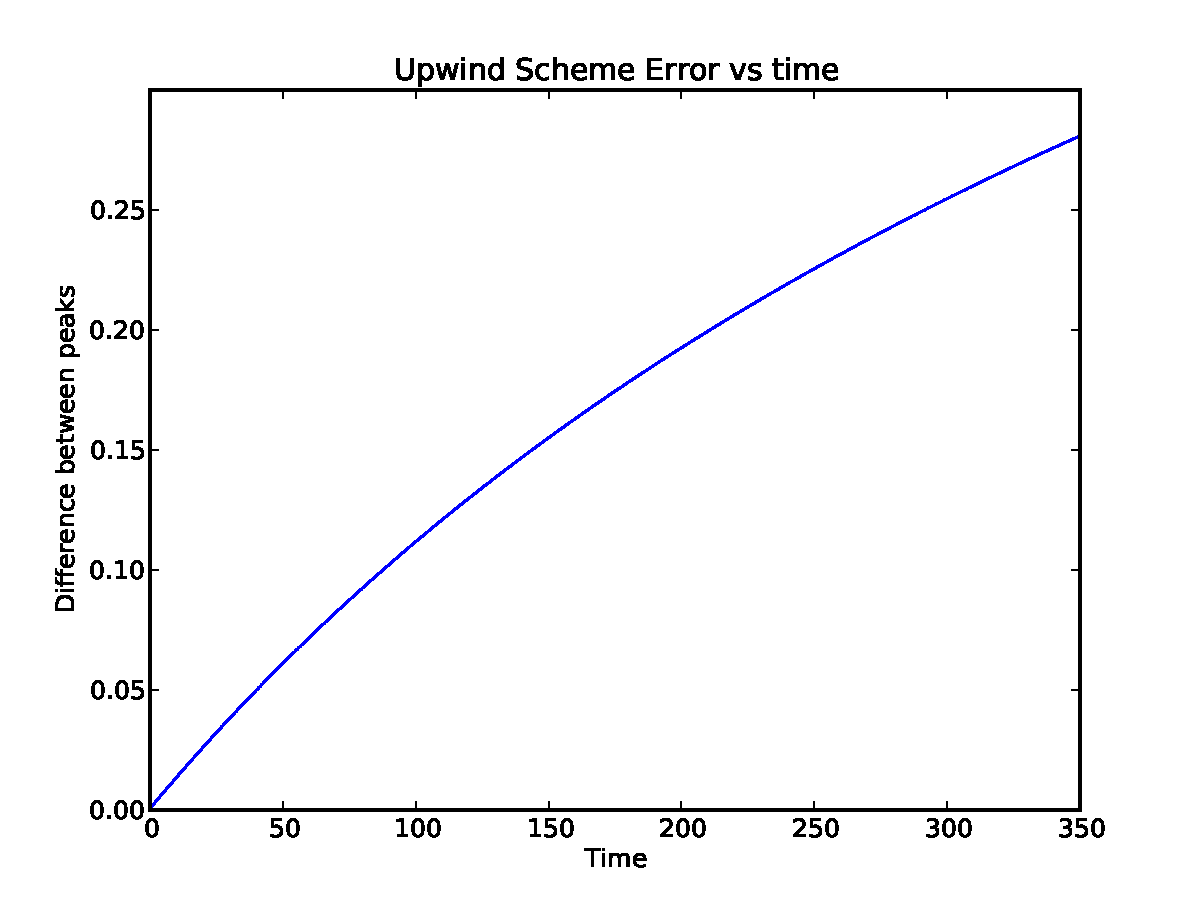
\includegraphics[width=0.7\textwidth]{error1.pdf}
\caption{Upwind scheme error for $\sigma = \sqrt{15}$ vs time.}
\label{fig:error1}
\end{figure}

To see what happens to the error if we change the analytic form of the Gaussian, we
replace $\sigma = \sqrt{15}$ with one $5$ times smaller, $\sigma = \sqrt{15}/5$. Running
the same code, we see that the with a smaller $\sigma$, the scheme's Gaussian drops
off more quickly, achieving larger errors at smaller times. However, as shown
in figure~\ref{fig:error2}, it stll moves at the same speed, reaching the 
boundary of $x = 100$ at the same time as before.

\begin{figure}[bth]
\centering
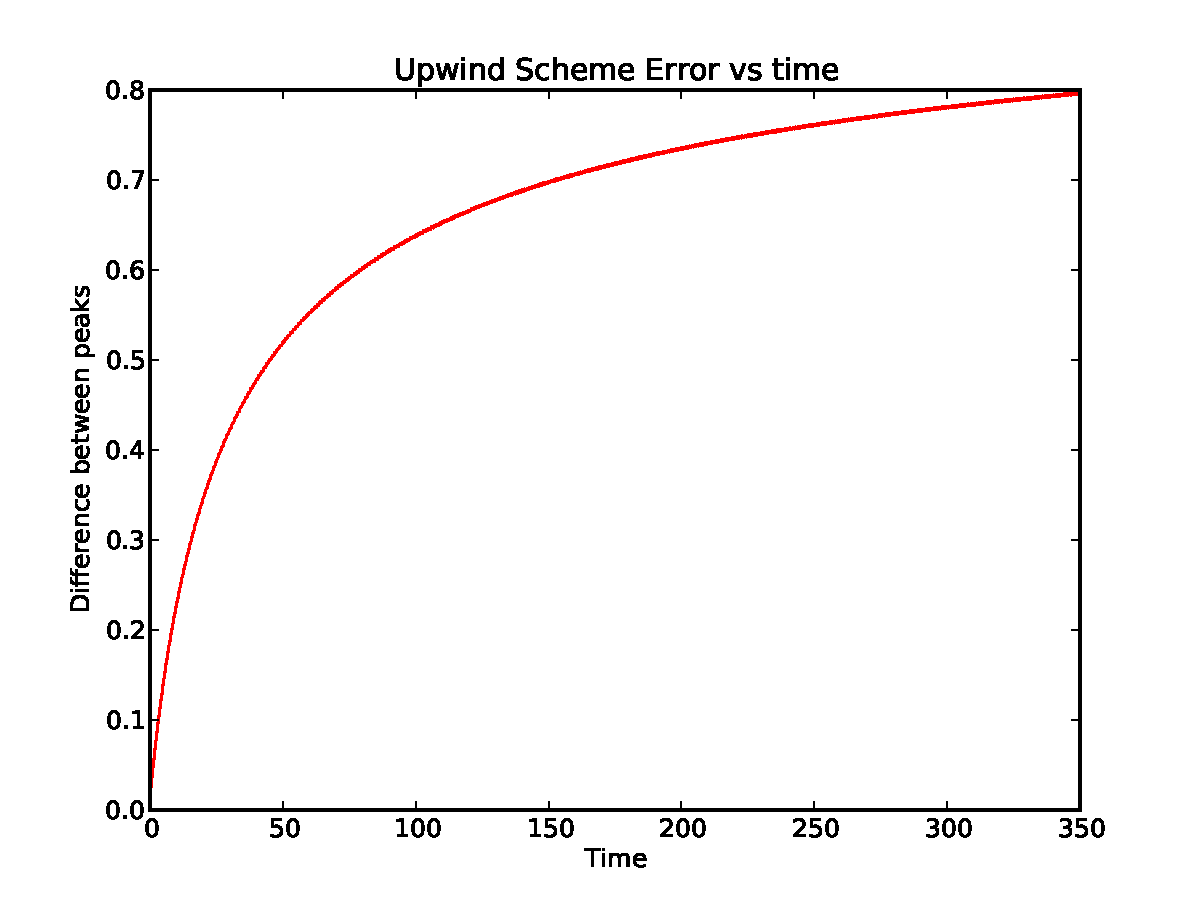
\includegraphics[width=0.7\textwidth]{error2.pdf}
\caption{Upwind scheme error for $\sigma = \sqrt{15}/5$ vs time}
\label{fig:error2}
\end{figure}

Both of the errors here are clearly not linear. To see what form the might have,
we make a log-log plot and notice that, for smaller t, the error is linear on that
plot with a slope of about $4/5$. So, for smaller t, the error goes as $t^{4/5}$. 

\begin{figure}[bth]
\centering
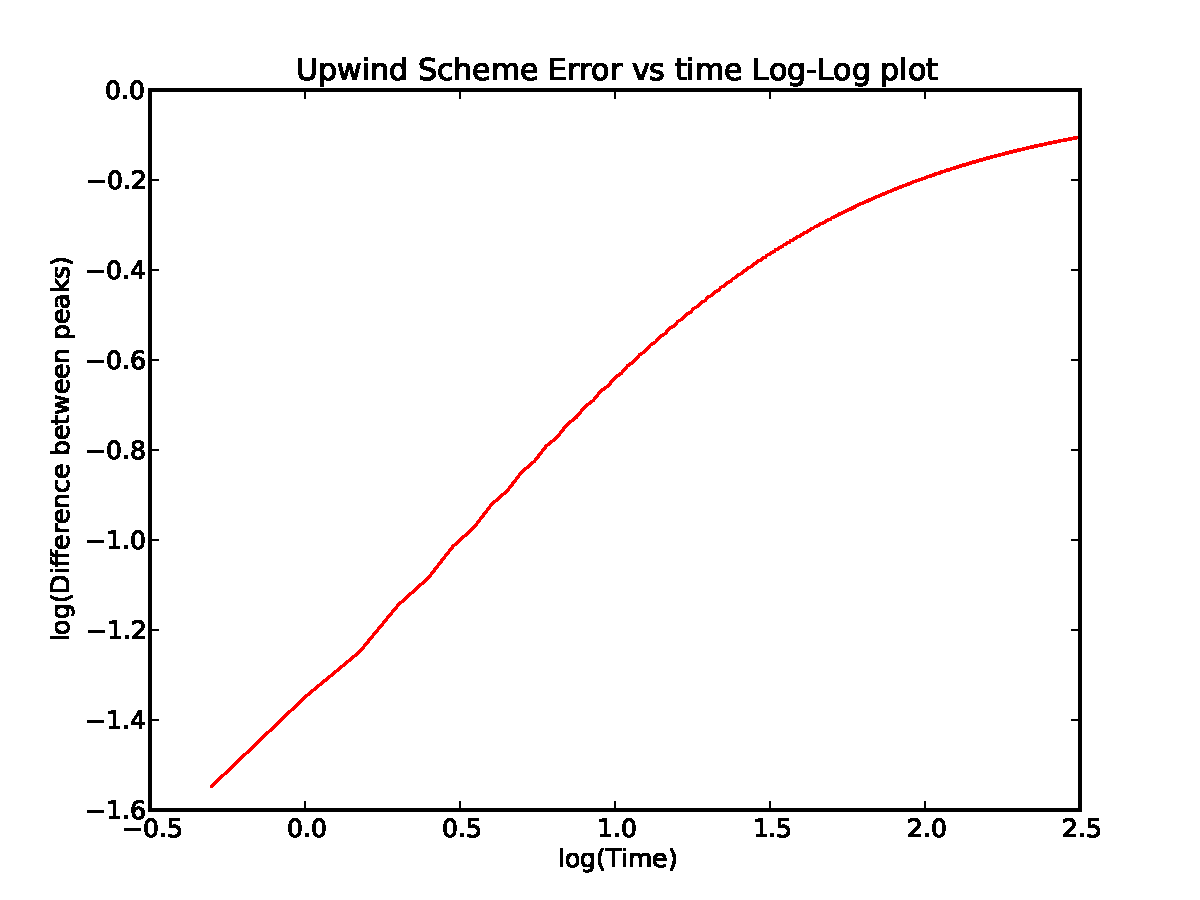
\includegraphics[width=0.7\textwidth]{error2log.pdf}
\caption{Log-log plot of Upwind scheme error for $\sigma = \sqrt{15}/5$ vs time}
\label{fig:error2log}
\end{figure}

For larger t, a plot of error vs log(t) (figure~\ref{fig:error2logt} looks more linear for larger t, indicating
that the error goes as the log of the time for larger t.

\begin{figure}[bth]
\centering
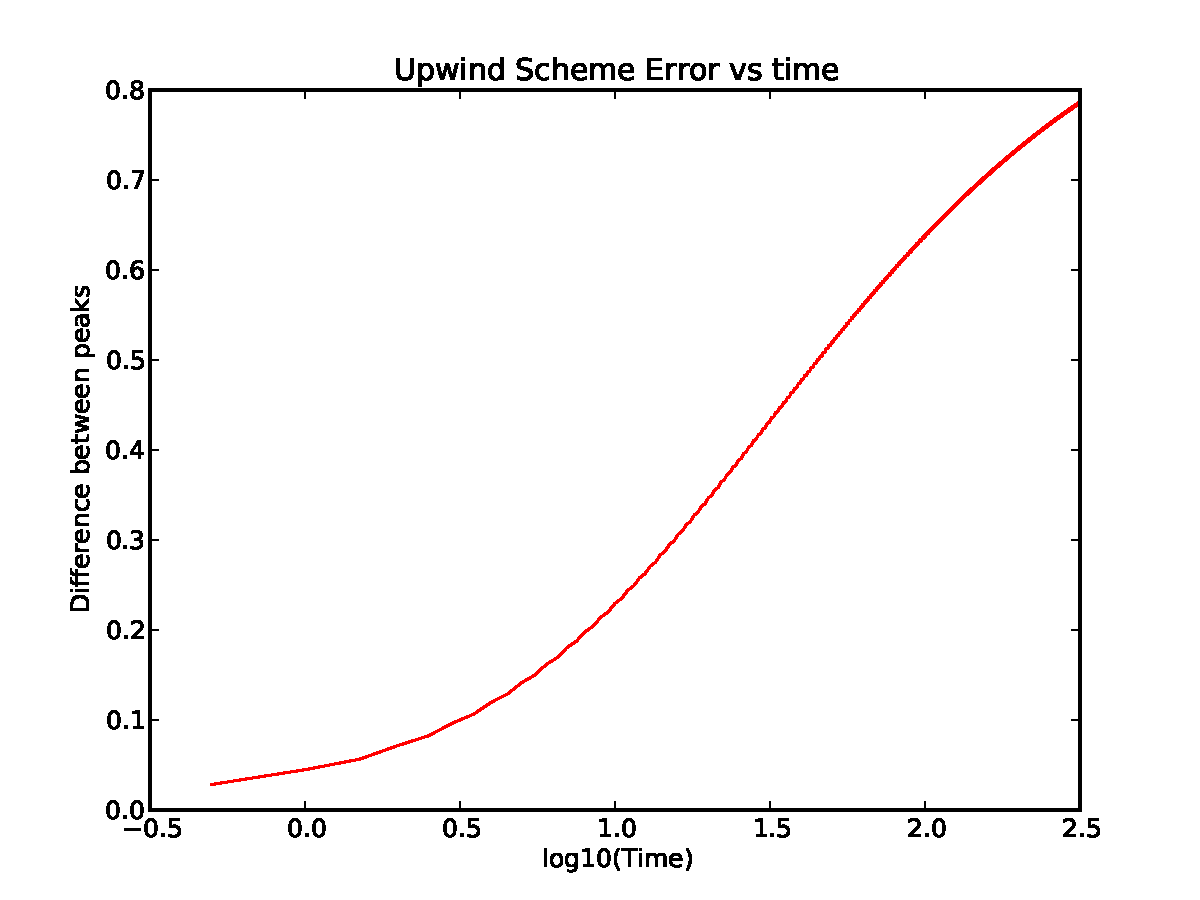
\includegraphics[width=0.7\textwidth]{error2logt.pdf}
\caption{Upwind scheme error for $\sigma = \sqrt{15}/5$ vs log(time)}
\label{fig:error2logt}
\end{figure}

\section{}

I'm confused about the implementation of the unstable FTCS scheme. I used the lines
\lstinputlisting[language=Python, firstline=67, lastline=67]{ws11.py}
\lstinputlisting[language=Python, firstline=70, lastline=71]{ws11.py}
and 
\lstinputlisting[language=Python, firstline=76, lastline=76]{ws11.py}
like before, but the scheme only seemed to maintain the same peak height and overall width
as the analytic solution, but just move forward at a faster speed. I didn't notice any 
instability except even at large times. However, I did notice, for the smaller sigma, some 
instability in the FTCS scheme: like the upwind scheme when $c_{CFL} < 0$, the gaussian
became oscillatory after many iterations.

\section{}

Implementing the Lax-Friedrich Method with the lines
\lstinputlisting[language=Python, firstline=67, lastline=67]{ws11.py}
\lstinputlisting[language=Python, firstline=72, lastline=73]{ws11.py}
and 
\lstinputlisting[language=Python, firstline=77, lastline=77]{ws11.py}
we get a very similar result that the upwind scheme gives. The behavior
of a decreasing peak and inreasing width is the same, which we can see by
comparing figure~\ref{fig:errorlax} to figure~\ref{fig:error1}. The graphs look almost 
identical. However, the Lax-Friedrich method reaches almost twice the error in half 
the time. That is, its peak decreases in height twice as fast, and it moves to the right
at twice the speed.

\begin{figure}[bth]
\centering
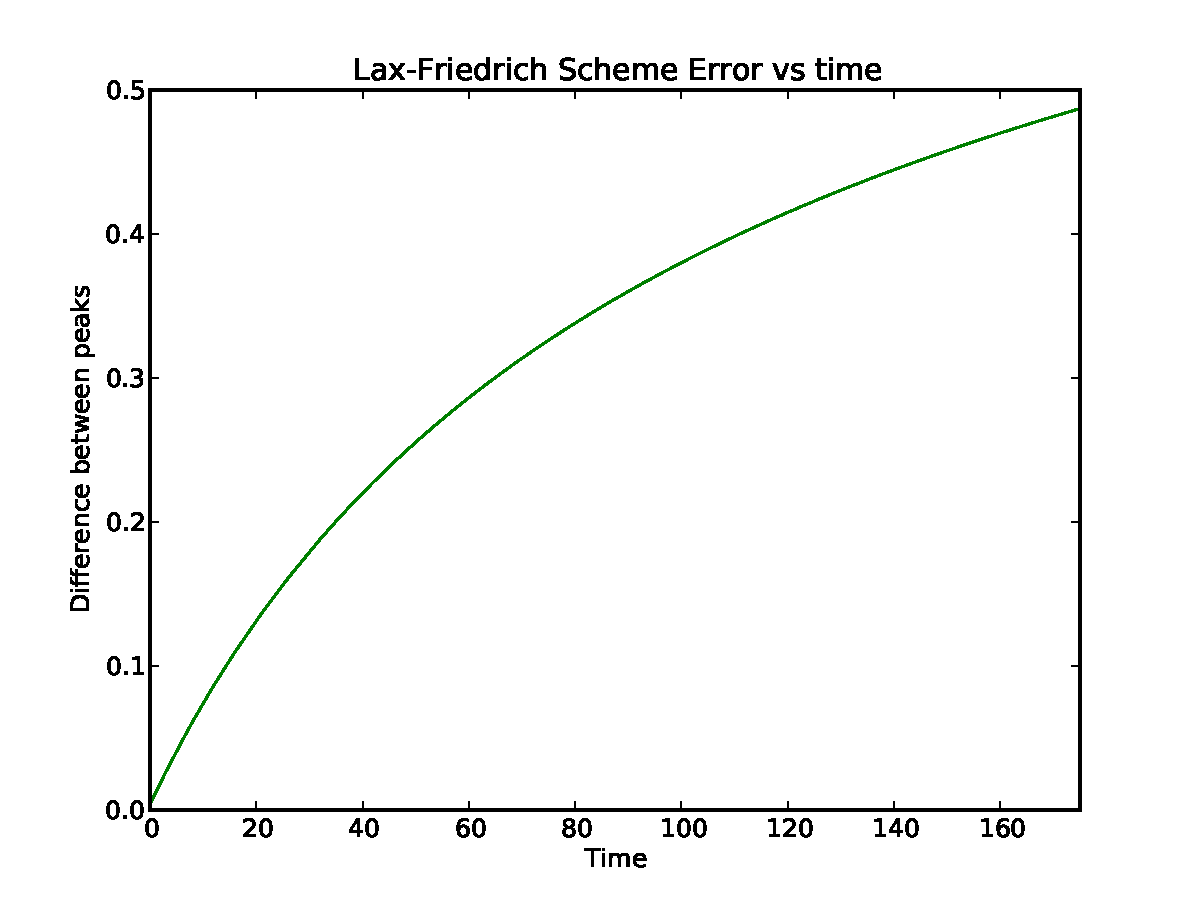
\includegraphics[width=0.7\textwidth]{error-lax.pdf}
\caption{Lax-Friedrich scheme error for $\sigma = \sqrt{15}$ vs time}
\label{fig:errorlax}
\end{figure}

\end{document}
